\documentclass[a4paper,twoside]{article}

\usepackage{epsfig}
\usepackage{subcaption}
\usepackage{calc}
\usepackage{amssymb}
\usepackage{amstext}
\usepackage{amsmath}
\usepackage{amsthm}
\usepackage{multicol}
\usepackage{pslatex}
\usepackage{algorithm2e}
\usepackage[bottom]{footmisc}
% Please add other packages that you may need BEFORE the SCITEPRESS.sty package.
\usepackage{natbib}
\usepackage{multirow}
\usepackage{SCITEPRESS}

\begin{document}

\title{Analysis of Programming Students' Prompts to Identify Interactions
Patterns with Generative AI}

\author{\authorname{Rodrigo Prestes Machado\sup{1}\orcidAuthor{0000-0003-0428-6387},
Carlos Alario Hoyos\sup{2}\orcidAuthor{0000-0002-3082-0814} and
Carlos Delgado Kloos\sup{2}\orcidAuthor{0000-0003-4093-3705}}
\affiliation{\sup{1}Department of Informatics, Federal Institute of Education,
Science and Technology, Porto Alegre, Brazil}
\affiliation{\sup{2}Department Telematics Engineering, Carlos III University,
Madrid, Spain}
\email{\ rodrigo.prestes@poa.ifrs.edu.br, \{calario,cdk\}@it.uc3m.es}
}

\keywords{Generative Artificial Intelligence, Programming Education, Chatbots}

\abstract{The abstract should summarize the contents of the paper and should
contain at least 70 and at most 200 words. The text must be set to 9-point font
size.}

\twocolumn\maketitle\normalsize\setcounter{footnote}{0}

\section{\uppercase{Introduction}}
\label{sec:introduction}

%What is the problem to be solved?

Recent advancements in Generative Artificial Intelligence (GenAI) have opened
up new possibilities in education. In programming courses, students can utilize
GenAI tools to improve their understanding, receiving assistance, feedback, and
detailed explanations.

The study of \cite{chan23} revealed that both undergraduate and postgraduate
students exhibit positive attitudes toward the use of GenAI in teaching and
learning, noting that it enhances the depth of their thinking and understanding.
Additionally, a systematic review conducted by \cite{Lo24} demonstrated that
students could effectively learn from ChatGPT, leading to improved understanding
and academic achievement. Besides of that, it was also observed that ChatGPT
enables students to regulate their learning pace, promoting self-regulation
\citep{Baha24} \citep{cai23}.

In the other hand, researchers have concerns about the impact of these
tools on students. The systematic review of \cite{Murillo23} indicated that
ChatGPT use might lead to an overreliance on the tool. \cite{chan23} also noted
that this reliance could result in a decrease in critical thinking, as students
might make decisions based solely on the information provided by ChatGPT.

The student's confidence is warranted, as shown by \cite{Puryear22}, who
demonstrated that GitHub Copilot can generate solutions for student assignments
with accuracy rates ranging from 68\% to 95\%. However, this raises concerns that
students might rely too heavily on GenAI tools, potentially neglecting a deeper
understanding of the underlying concepts. \cite{cai23} further identified
overdependence and reduced intellectual engagement as significant drawbacks of
using ChatGPT in learning.

Regardless of teachers' preferences or beliefs, a preliminary surveys performed
by \cite{Dickey24} revealed that at least 54.5\% of students are already using
GenAI for homework. This highlights the need to understand how students are
interacting with these tools and how they can be used to enhance learning.
Furthermore, a review by \cite{Lo24} emphasized the necessity for extended
studies and objective measures to gather more robust evidence on the use of
GenAI tools in education.

% Are there any existing solutions?

To deal with this issue, some researchers have proposed different pedagogical
strategies \cite{Denny24} introduced the concept of \textit{Prompt
Problems}, where students solve programming exercises by formulating natural
language prompts. \cite{Prasad24} proposed a self-regulated learning framework
using GenAI to solve programming problems. \cite{Lauren23} explored the
integration of GenAI with evidence-based learning strategies in computer science
and engineering courses.

% Which is the best?

The study of effective educational strategies in use of GenAI tools in education
context are important for determining the best training for educators. However,
as these tools gain popularity among students \cite{Dickey24} the urgency to
equip educators with best practices may lag behind their rapid adoption.
Therefore, analyzing students' interaction patterns with GenAI tools is
important for understanding how these tools are being used and how educators can
leverage them to enhance learning. In addition, these interaction patterns can
create new opportunities to redesign GenAI tools to better support pedagogical
strategies without repressing the development of abstract, critical and creative
thinking.

% What is its main limitation?

Nevertheless, it is important to consider how GenAI tools affect students across
different demographic groups, knowledge areas, cultural backgrounds
\cite{catalan21} \cite{neo22} and students' prior experience. Thus, this works
is limited to a specific group of students and a specific GenAI tool. The
results may not be generalizable to other populations or tools.

% What do you hope to achieve?

This study aims to analyze the interactions between students and CharlieBot,
an ChatGPT 3.5 based bot developed by UC3M that leverages Retrieval-Augmented
Generation (RAG) to enhance its contextual understanding of Java programming.

\section{\uppercase{Related Work}}

The advancements in GenAI and its use in programming courses have raised
possibilities and concerns among educators and researchers. The study of
\cite{Yilmaz23} found that the main benefit of using ChatGPT in programming
learning is to provide providing fast and mostly correct answers to questions,
improving thinking skills, facilitating debugging, and increasing
self-confidence. In contrast, the study the same appoint limitations such ask
laziness, being unable to answer some questions, or giving incomplete/incorrect
answers, causing professional anxiety in students.

From a cognitive perspective, \cite{Lo24} shown that students were able to
learn from ChatGPT, which increased their understanding and achievement.
However, concerns were raised that the growing use of AI tools might lead to a
decline in critical thinking among students. Teachers and stakeholders should
continue to investigate pedagogical approaches that leverage ChatGPT to enhance
students' understanding and critical thinking. For example, teachers can
instruct students to fact-check and validate information produced by ChatGPT.

Examined students from different demographic groups using AI tools like
ChatGPT, comparing perceptions and impacts among these groups. The results
showed that AI tools had a positive impact on academic performance, especially
for students with less prior experience.

% Critical thinking is a fundamental skill for students to develop, as it enables
% them to analyze, evaluate, and synthesize information. This skill is essential
% for problem-solving and decision-making, making it a crucial aspect of
% educational success, specifically in programming courses. However, the use of AI
% tools like ChatGPT has raised concerns about the potential impact on students'
% critical thinking abilities \cite{Murillo23} \cite{cai23} \cite{chan23}.

% In the other hand, the study of \cite{zhang24} suggested that incorporating
% ChatGPT could stimulate students' critical thinking, probably because they
% had to assess the correctness of ChatGPT's answers.

% Regarding self-regulation, \cite{cai23} noted that ChatGPT allowed students to
% regulate their learning pace.

% \cite{wu24} found that ChatGPT-supported learning not only promoted students'
\begin{table*}[htbp]
  \caption{Categories - adapted from \cite{Ghimire24}}
  \begin{center}
    \renewcommand{\arraystretch}{1.5} % Increase the spacing between rows
    \begin{tabular}{|p{3,5cm}|p{11cm}|}
      \hline
      \textbf{Category} & \textbf{Description} \\
      \hline
      Debugging Help & Prompts that seek help to identify, fix errors, or understand the provided code snippet. \\
      Conceptual Question & Prompts that are more about understanding concepts than specific code. \\
      Student Correction & Prompts where the student corrects the bot. \\
      \hline
      Code Snippet & Prompts that ask for a specific part of the code, like a function or a segment. \\
      Complete Solution & Prompts that request an entire solution or a complete code snippet. \\
      Multiple Question & Prompts where the user wants to solve a multiple-question exercise (Quiz). \\
      \hline
      Language Change & Prompts that request a change of idiom. \\
      Uncategorized & Prompts that do not fit into any of the above categories. \\
      \hline
    \end{tabular}
    \label{tab:categories}
  \end{center}
\end{table*}

\subsection{Metacognition}

The use of GenAI tools can help students learning by providing rapid assistance
and feedback. However, it is important to teach students how to use these tools
properly to promote learning. In this sense, it is important that students are
aware of the cognitive processes.

Metacognition is defined as the awareness about the cognitive processes.
\cite{flavell79} defined a model of cognitive monitoring in four classes of
phenomena that can act or interact with each other, which are: Metacognitive
Knowledge, Metacognitive Experience, Metacognitive Task, and Metacognitive
Strategies. Metacognitive knowledge refers beliefs about what factor or
variables affect the course and outcome of cognitive enterprise. It is
subdivided into three majors categories or variables: Person, Task, and
Strategy. Metacognitive experience refers to the feelings and emotions
associated with cognitive activities. Metacognitive task refers to the type of
task or problem that the individual is facing. Metacognitive strategies refer to
the methods or techniques that individuals use to control their cognitive
processes.


\subsection{CharlieBot}

CharlieBot is a ChatGPT 3.5 based bot that provides assistance to students in a
Java programming courses at UC3M. The bot uses the content of UC3M Java
programming course at EdX to supply a RAG(Retrieval-Augmented Generation) system
and thus try to respond more accurately to students' questions \cite{Sun24}. The
main goal of CharlieBot is support students in their learning process by
providing personalized assistance and feedback.

\section{\uppercase{Method}}

The study was conducted in three phases: data collection, categorization, and
analysis. During the first semester of 2024, student interactions with
CharlieBot were collected as part of the Java programming course at UC3M.
The categorization phase involved classifying student messages into eight
categories. The table \ref{tab:categories} shows the categories of analysis and
their description. The initial categories were based on the work of
\cite{Ghimire24}, however, four new categories were added due to the need to
give more detail to the classification. The analysis phase involved to
understand the way that the students interact with CharlieBot.
\section{\uppercase{Results and Discussion}}

The Figure \ref{fig:graph1} shows the distribution of the messages in the
categories:

\begin{figure}[h!]
    \centering
    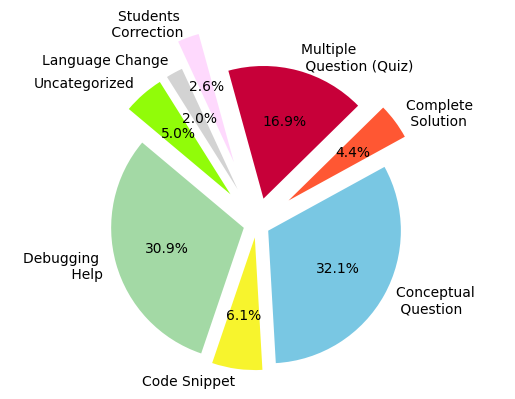
\includegraphics[scale=0.62]{img/figure1.png}
    \caption{Classification of messages.}
    \label{fig:graph1}
\end{figure}

\begin{figure*}[htbp]
  \centering
  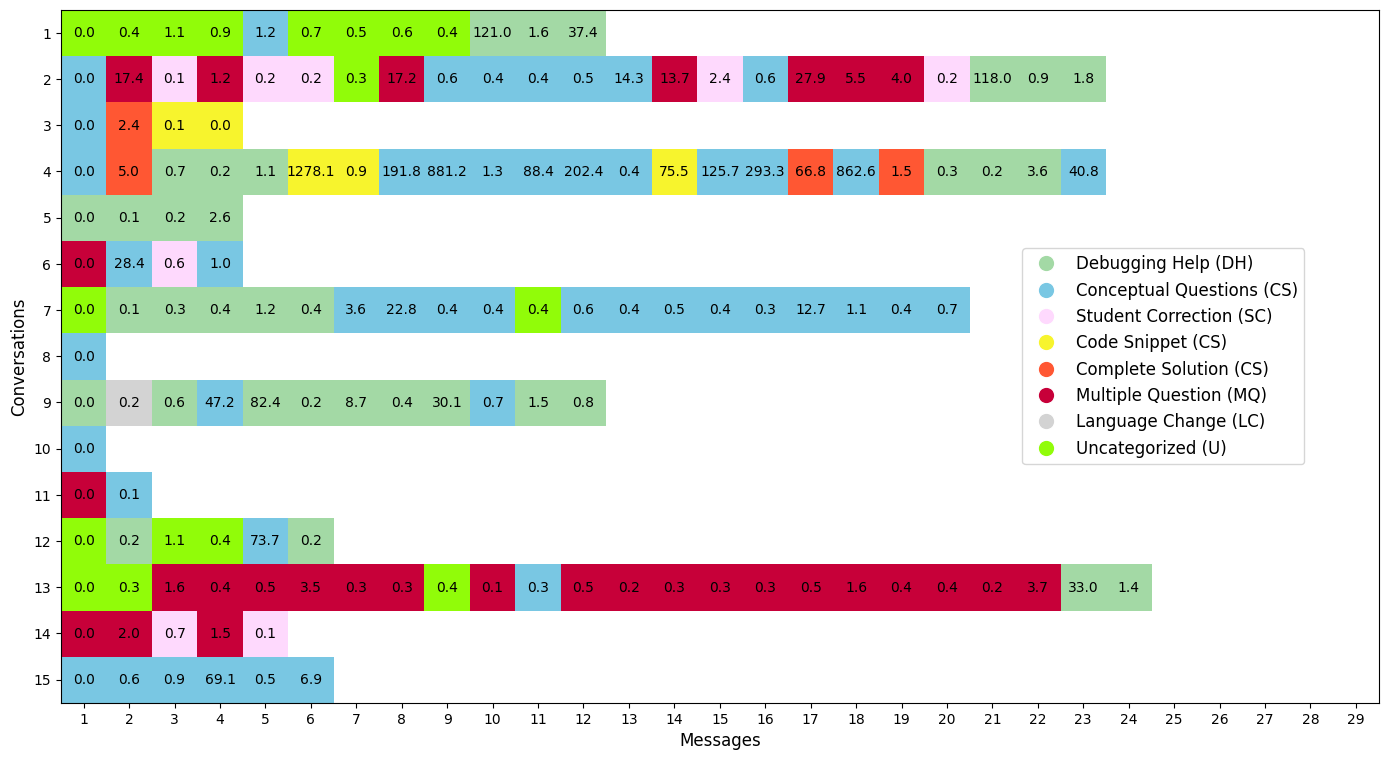
\includegraphics[scale=0.52]{img/figure2.png}
  \caption{Examples of conversations.}
  \label{fig:graph2}
\end{figure*}

% Approximately 64\% of the messages pertain to categories associated with
% critical thinking, corroborating with the findings of
% \cite{Ghimire24}. In contrast, around 28\% of the messages
% indicate a preference among students for ready-made answers.

% Since most of the messages are located in categories where students are 
% notoriously more active in their learning (conceptual questions 32.1% and 
% Debugging Help 30.9%), it seems that students are trying to use the AI in a 
% way that promotes their learning. However, the pattern of conversations with 
% sequential blocks and also little spacing may suggest that there is a gap in 
% knowledge of study strategies.

% Uncategorized

The Figure \ref{fig:graph1} shows that around 5\% of the prompts
written by students were not categorized. These messages range from
greetings to the Bot, such as a simple "\textit{Hola}," to
contextual statements like "\textit{Estoy repasando orientación a
objetos.}"

% Multiple Choice
\subsubsection*{Sequence of Multiple Choice}

Around 16.9\% of the messages were classified as Multiple Choice. These prompts
typically involve students sending one or more exercises to CharlieBot, asking
for the solution.

We identified a sequence of Multiple Choice patterns in some of the
conversations. From the point of view of Metacognitive Knowledge, a possible
interpretation of this complex phenomenon is that students may believe in their
inability to answer several questions. They may also assume that the questions
share a common theme, and solving them together may help consolidate knowledge.
Additionally, they might understand that obtaining the answers quickly is more
efficient.

Regarding Metacognitive Experiences, students may experience feelings such as
cognitive overload, a sense of urgency, and/or confidence in ready-made answers,
which can often lead to relief and a reduction of frustration.

Concerning the Metacognitive about the Task, one interpretation may be that the
student simply wants to complete the task quickly to alleviate the workload,
and/or obtain a correct answer without focusing on deeper learning at
this moment.

In relation to Metacognitive Strategies, students are likely focusing on saving
time and/or possibly lacking planning skills. They may also perceive that
solving the questions on their own requires too much cognitive effort, but this
pattern might reveal a lack of progress monitoring and understanding of
concepts. After obtaining the answers, the metacognitive evaluation process
could lead to feelings of satisfaction, but further reflection may indicate that
the strategy was not effective in supporting deep learning. Depending on this
evaluation, it may influence future decision-making to change the strategy.

% Debugging help
\subsubsection*{Sequence of Debugging Help}

Around 30.9\% of the messages were classified as Debugging Help. Besides of
that, we identified a pattern of a sequences of Debugging Help in the
conversations. These prompts typically start with a message requesting a
Complete Solution or a Code Snippet. After that, the students normally chance
from passive to more active learning strategy.

In terms of Metacognitive Knowledge, the student probably recognizes that they
do not have the necessary tools or knowledge to debug the code on their own.
Concerning the understanding of the task, they may know that debugging is not
just a matter of superficial corrections but requires understanding the
underlying logic. Thus, the student apparently believes that the sequence of
questions related to debugging will help them understand the codes.

In terms of Metacognitive Experiences, some feelings may arise at this moment,
such as frustration or uncertainty in the face of errors, confusion during the
process, and also growing confidence or satisfaction as they better understand
the code and possible corrections.

With respect to Metacognitive related with the objective of the Task, the
student is probably focused on understanding the code in practical terms,
identifying errors, and learning how to better debug in the future.

As for Metacognitive associated with the Strategy, the student has requested
external help and realizes that dividing the debugging task into several
questions can result in a better understanding of the code. They can monitor
their progress throughout the process, adjusting their questions as necessary,
evaluate the effectiveness of the responses received, and reflect on what was
learned during the process.

\begin{figure*}[htbp]
  \centering
  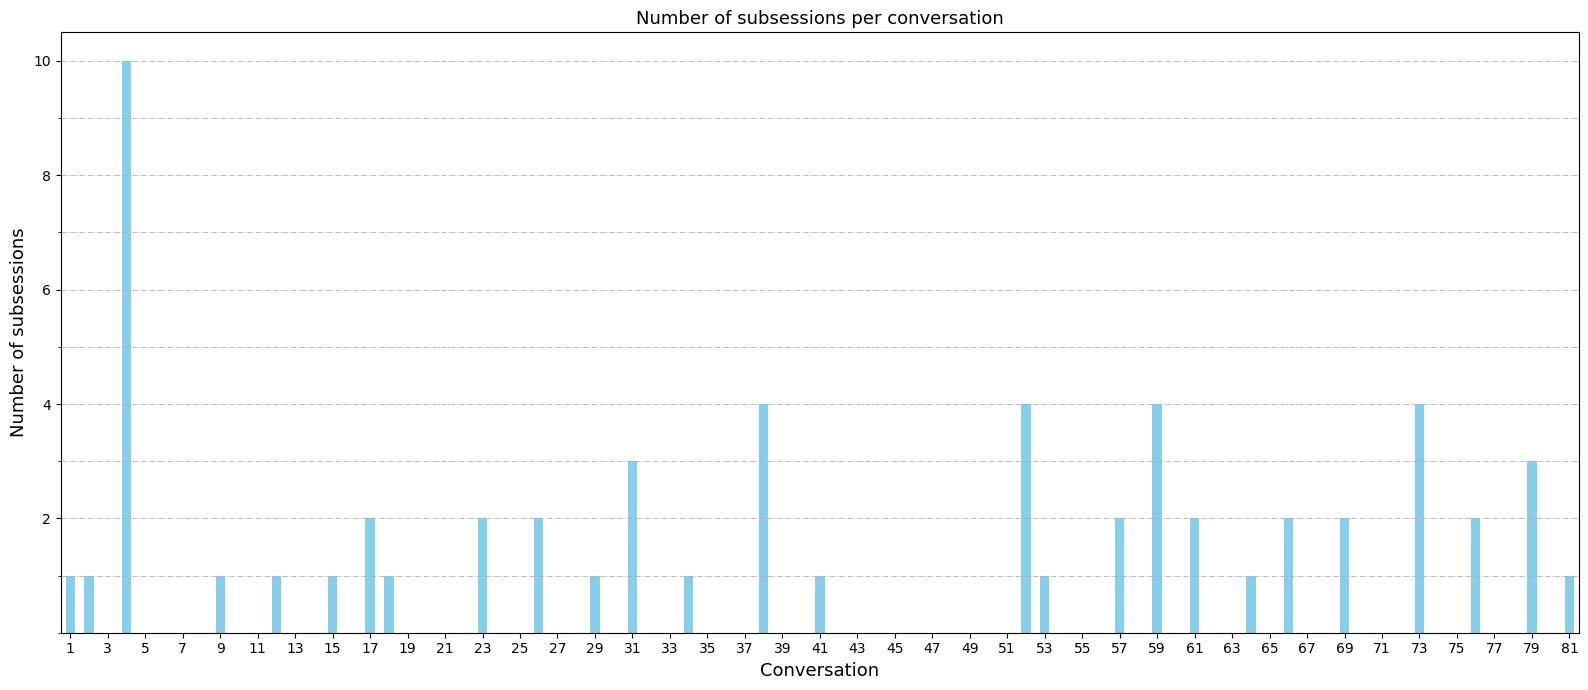
\includegraphics[scale=0.55]{img/figure3.png}
  \caption{Interaction times per categories.}
  \label{fig:graph3}
\end{figure*}

% Conceptual Questions
\subsubsection*{Sequence of Conceptual Question}

Messages classified as conceptual questions represent around 32\% of all
messages. We have found a pattern of sequences of Conceptual Questions in some
conversations. Some conversations are entirely composed of messages classified
as Conceptual Questions. In other cases, the sequence of Conceptual questions
starts with a request for a Complete Solution or a Code Snippet, followed by
a progression of Conceptual Questions. In both cases, the student is actively
engaging with the bot to understand the concepts and compromised with more
deep learning.

Regarding Metacognitive Knowledge, these sequences of prompts classified as
Conceptual Question, can be interpreted that the students are aware they have
not fully mastered a concept and are trying to understand it, demonstrating a
good level of self-awareness. In this sense, the student realizes that the
problem requires an understanding of concepts in order to advance in their
studies. In this way, the student applies an active learning strategy.

About Metacognitive Experience, several types of feelings may be associated at
this moment, such as actively reflecting on the answers, uncertainty and/or
confusion when trying to understand the concept, frustration for not
progressing, and satisfaction as their questions are answered in a way that
facilitates understanding.

Regarding the type of Metacognition related to objective of the Task, the
students may recognize the difficult and trying to achieve a deeper
understanding of the evolved concepts to later apply in practice.

With respect to Metacognitive Strategies, the student demonstrates a sence of
planning to identify their knowledge gaps. They may start with more general
questions to obtain an overview of the concept and then ask more specific
questions as they gain more clarity. Because the questions are in sequence, the
student probably can adequately monitor their progress.

\subsection*{Interleaving}

% Interleaving

Intervealing is a study strategy that involves mixing or alternating different
topics or problems within a single learning session. This
approach has been shown to be useful for promoting long-term learning and
improving the application of knowledge in other situations \cite{Rivers21}.

When analyzing the classification of messages in conversations, we identified
the presence of sequences of messages belonging to the same category, that it
could suggest a low occurrence of interleaving. To better assess the extent of
these sequences, we calculated the percentage of messages that were part of
repeated blocks.

Considering blocks with at least three messages, we observed that 56.2\% of the
students' prompts were grouped into some sequence. When analyzing blocks with a
minimum of 4 messages, we found that 47.5\% of the prompts were part of
continuous sequences. These results indicate a moderate incidence of
interleaving among the students' messages.

To illustrate the presence of blocks the Figure \ref{fig:graph2} presents
examples of conversations and their classification. In Conversation 2, the
student alternates messages among Code Snippet, Debugging Help and Conceptual
Question, showing an tendency of interleaving between practical and theoretical
perspectives. In contrast, in Conversation 10, the student focused on a single
block of Conceptual Question. Although the focus was on understanding a
theoretical concept, this conversation tended not to promote interleaving, due
to the absence of alternation between different types of tasks.


\subsection*{Spacing}

% Spacing
Spacing, a well-established learning strategy \cite{Carvalho20}, was examined
by analyzing the time intervals between users’ interactions with CharlieBot.
Although only 7.4\% of the conversations exhibited message delays exceeding 24
hours, 26.19\% involved response times longer than 60 minutes. These findings
suggest that students typically do not extend conversations across multiple days.
However, the data also reveal that some conversations had one or more pauses
exceeding an hour, a practice known to enhance knowledge retention.

% Another interesting study technique is spacing. Only 7.4% of the conversations
% exhibited message delays exceeding 24 hours and 26.19% involved response times 
% longer than 60 minutes. However, Carlos told me that this may be due to some 
% limitation of the bot, as it only maintains a conversation while the browser 
 % tab is open.




 % There is a big difference (I haven't looked at it statistically yet) in the 
%  interaction time with the Bot when a student asks conceptual questions. 
%  Perhaps this actually makes sense, since it is a category where, from the 
%  point of view of the metacognitive objective, the student is more concerned 
%  with understanding a concept and deeper learning.

\section{Conclusion}

The results of this study suggest that students interact with CharlieBot in a
manner that promotes critical thinking. The majority of the messages analyzed
were related to debugging help, conceptual questions, and student correction,
indicating that students are actively engaging with the bot to understand
concepts and solve problems. This is a positive outcome, as it suggests that
CharlieBot is being used as a tool to enhance learning rather than a crutch for
students to rely on.

\section*{ACKNOWLEDGEMENTS}

The authors would like to thank the Federal Institute of Education, Science and
Technology (IFRS) for the partial financial support provided for the execution
of this research.

\bibliographystyle{apalike}
{\small
\bibliography{References}}

\section*{\uppercase{Appendix}}

If any, the appendix should appear directly after the
references without numbering, and not on a new page. To do so please use the
following command: \textit{$\backslash$section*\{APPENDIX\}}

\end{document}

